\section{Avaliação de desempenho e funcionalidade}
Nessa sessão será apresentado os ambientes dos cenários de testes, principalmente como foram configurados e seus respectivos \textit{hardwares}. Também será exposto os resultados dos experimentos realizados neste trabalho.
\subsection{Equipamentos}

Como explicado na seção \ref{Metodologia}, o testes serão realizados seguindo cenários com diversos equipamentos, que devem realizar funções diferentes dependendo do cenário selecionado.
A coleta de métricas de consumo de processador, memória, entrada e saída de \textit{bits} pela interface de rede
foram realizadas usando o \textit{software} Prometheus em conjunto com o Grafana para a visualização gráfica dos dados.

\begin{table}[H]
\centering
\label{tab:freq-conf}
\begin{tabular}{cc|}
\hline
\rowcolor[HTML]{DFDFDF} 
\multicolumn{2}{|c|}{\cellcolor[HTML]{DFDFDF}A - Thinkpad T440s}               \\ \hline
\rowcolor[HTML]{EFEFEF} 
\multicolumn{1}{|c|}{\cellcolor[HTML]{EFEFEF}Processador}         & Intel\textregistered\space Core\texttrademark\space i5 4200U          \\ \hline
\multicolumn{1}{|c|}{RAM}                    & 8GB DDR3               \\ \hline
\rowcolor[HTML]{EFEFEF} 
\multicolumn{1}{|c|}{\cellcolor[HTML]{EFEFEF}SO} & NixOS GNU/Linux                   \\ \hline
\multicolumn{1}{|c|}{\textit{kernel}}                   & 6.1.79          \\ \hline \hline
\rowcolor[HTML]{DFDFDF} 
\multicolumn{2}{|c|}{\cellcolor[HTML]{DFDFDF}B - Raspberry Pi 4}                 \\ \hline
\rowcolor[HTML]{EFEFEF} 
\multicolumn{1}{|c|}{\cellcolor[HTML]{EFEFEF}Processador} & Broadcom BCM2711 \\ \hline
\multicolumn{1}{|c|}{RAM} & 4GB LPDDR4  \\ \hline
\rowcolor[HTML]{EFEFEF} 
\multicolumn{1}{|c|}{\cellcolor[HTML]{EFEFEF}SO}                 & RPiOS Lite GNU/Linux     \\ \hline
\multicolumn{1}{|c|}{\textit{kernel}}   & 6.6.20+rpt-rpi-v8    \\ \hline 
\end{tabular}
\begin{tabular}[h]{cc|} \hline
\rowcolor[HTML]{DFDFDF} 
\multicolumn{2}{|c|}{\cellcolor[HTML]{DFDFDF}C - \textit{Custom Build}}              \\ \hline
\rowcolor[HTML]{EFEFEF} 
\multicolumn{1}{|c|}{\cellcolor[HTML]{EFEFEF}Processador} & Intel\textregistered\space Xeon\textregistered\space E5-2670v3            \\ \hline
\multicolumn{1}{|c|}{RAM}                         & 16GB DDR4 ECC              \\ \hline
\rowcolor[HTML]{EFEFEF} 
\multicolumn{1}{|c|}{\cellcolor[HTML]{EFEFEF}SO}         & NixOS GNU/Linux \\ \hline
\multicolumn{1}{|c|}{\textit{kernel}}           & 6.1.79  \\ \hline \hline
\rowcolor[HTML]{DFDFDF} 
\multicolumn{2}{|c|}{\cellcolor[HTML]{DFDFDF}D - TPLink WR741ND}                 \\ \hline
\rowcolor[HTML]{EFEFEF} 
\multicolumn{1}{|c|}{\cellcolor[HTML]{EFEFEF}Banda} & \textit{FastEthernet} 100Mbit/s         \\ \hline
\multicolumn{1}{|c|}{\textit{Firmware}}                        & OpenWRT                \\ \hline
\rowcolor[HTML]{EFEFEF} 
\multicolumn{1}{|c|}{\cellcolor[HTML]{EFEFEF}Núm. Portas}         & 4        \\ \hline
\multicolumn{1}{|c|}{Lançamento}           & 2016    \\ \hline
\end{tabular}
\caption{Especificação dos Equipamentos}
\end{table}
%Para a realização dos cenários de testes foram criados \textit{testbeds} compostos por três computadores, um roteador e um \textit{switch}. 
%\subsection{\textit{Testbed}}
%Para a realização dos dois cenários de testes foi criado uma \textit{Testbed} composta por três máquinas rodando GNU/Linux.
%Todas as máquinas estam equipadas com interfaces de redes \textit{Gigabit} para maior banda de tranfêrencia. 


\subsubsection{Configuração dos Equipamentos}
No \textbf{cenário I} os equipamentos A e B foram configurados para receberem endereços \ac{IP} pelo serviço \ac{DHCP}.  

No \textbf{cenários II e III}, o roteador um ip estático assim como o segundo computador. O primeiro computador recebeu um endereço \ac{IP} dinâmico dado pelo roteador acima do roteador. 

Para o roteador: 

\begin{verbatim}
# No roteador
sudo systemctl net.ipv4.ip_forward 
sudo ip addr add 10.0.1.1/24 dev {iface1} 
sudo iptables -t nat -A POSTROUTING -o {iface2} -j MASQUERADE 
\end{verbatim}

\begin{verbatim}
# No segundo computador
sudo ip addr add 10.0.1.2/24 dev {iface}
sudo ip route add 192.168.0.0/24 via 10.0.1.1 dev {iface}
\end{verbatim}

Já no \textbf{cenário IV} o roteador também foi configurado para receber um endereço dinâmico na porta \ac{WAN} e fixo na porta \ac{LAN}. Toda configuração foi feita pela interface gráfica \textit{web} disponibilizada pelo \textit{OpenWRT}. O segundo computador não precisou ser configurado pois o mesmo ganhou endereço \ac{IP} dinâmico pelo servidor \ac{DHCP} do roteador.


\subsection{Throughput}


\begin{figure}[H]
    \centering
    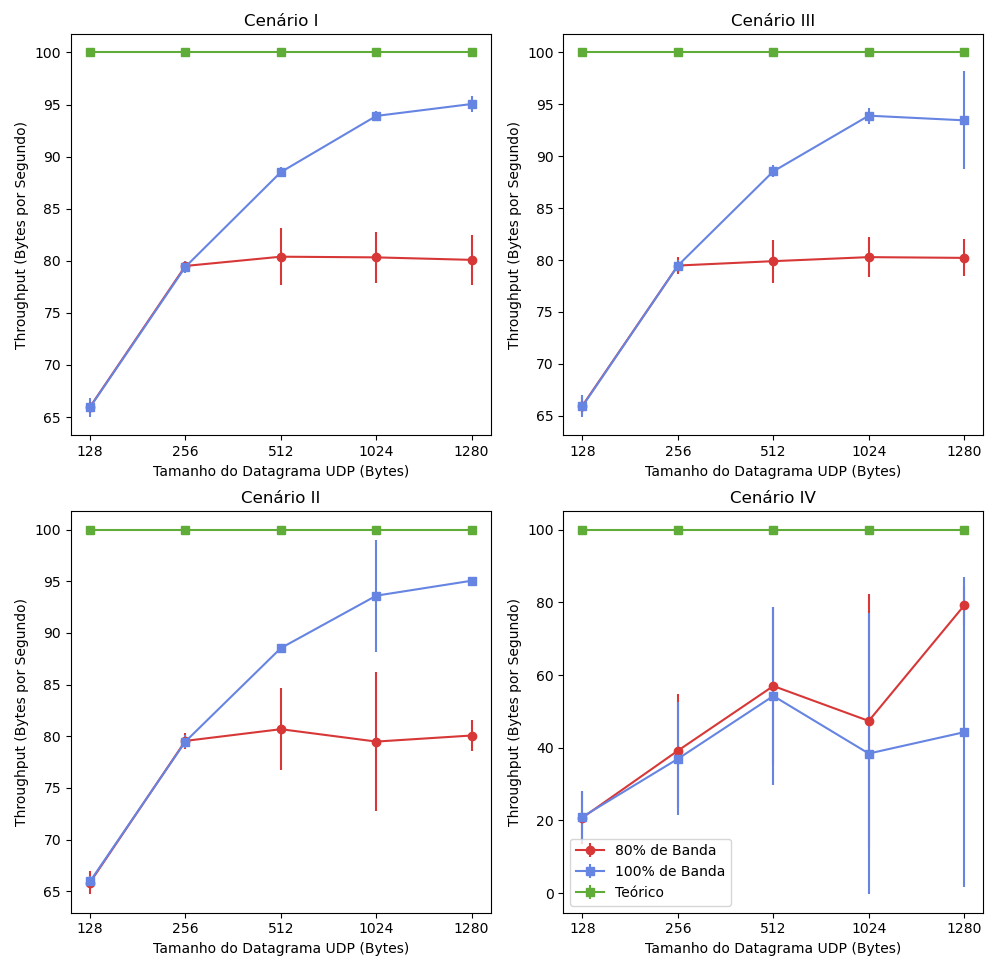
\includegraphics[width=0.9\linewidth]{sources/fig-throughput.png}
    \caption{Cenários dos testes a serem realizados.}
    \label{fig:cenarios}
\end{figure}




